%%%%%%%%%%%%%%%%%%%%%%%%%%%%%%%%%%%%%%%%%
% Short Sectioned Assignment LaTeX Template Version 1.0 (5/5/12)
% This template has been downloaded from: http://www.LaTeXTemplates.com
% Original author:  Frits Wenneker (http://www.howtotex.com)
% License: CC BY-NC-SA 3.0 (http://creativecommons.org/licenses/by-nc-sa/3.0/)
%%%%%%%%%%%%%%%%%%%%%%%%%%%%%%%%%%%%%%%%%

% \documentclass[paper=a4, fontsize=11pt]{scrartcl} % A4 paper and 11pt font size
\documentclass[11pt, a4paper]{book}
\usepackage[T1]{fontenc} % Use 8-bit encoding that has 256 glyphs
\usepackage[utf8]{inputenc}
\usepackage{fourier} % Use the Adobe Utopia font for the document - comment this line to return to the LaTeX default
\usepackage{listings} % para insertar código con formato similar al editor
\usepackage[spanish, es-tabla]{babel} % Selecciona el español para palabras introducidas automáticamente, p.ej. "septiembre" en la fecha y especifica que se use la palabra Tabla en vez de Cuadro
\usepackage{url} % ,href} %para incluir URLs e hipervínculos dentro del texto (aunque hay que instalar href)
\usepackage{graphics,graphicx, float} %para incluir imágenes y colocarlas
\usepackage[gen]{eurosym} %para incluir el símbolo del euro
\usepackage{cite} %para incluir citas del archivo <nombre>.bib
\usepackage{enumerate}
\usepackage{hyperref}
\usepackage{graphicx}
\usepackage{tabularx}
\usepackage{booktabs}
\usepackage{pdflscape}

\usepackage[table,xcdraw]{xcolor}
\hypersetup{
	colorlinks=true,	% false: boxed links; true: colored links
	linkcolor=black,	% color of internal links
	urlcolor=cyan		% color of external links
}
\renewcommand{\familydefault}{\sfdefault}
\usepackage{fancyhdr} % Custom headers and footers
\pagestyle{fancyplain} % Makes all pages in the document conform to the custom headers and footers
\fancyhead[L]{} % Empty left header
\fancyhead[C]{} % Empty center header
\fancyhead[R]{Elena Ortega Contreras} % My name
\fancyfoot[L]{} % Empty left footer
\fancyfoot[C]{} % Empty center footer
\fancyfoot[R]{\thepage} % Page numbering for right footer
%\renewcommand{\headrulewidth}{0pt} % Remove header underlines
\renewcommand{\footrulewidth}{0pt} % Remove footer underlines
\setlength{\headheight}{13.6pt} % Customize the height of the header

\usepackage{titlesec, blindtext, color}
\definecolor{gray75}{gray}{0.75}
\newcommand{\hsp}{\hspace{20pt}}
\titleformat{\chapter}[hang]{\Huge\bfseries}{\thechapter\hsp\textcolor{gray75}{|}\hsp}{0pt}{\Huge\bfseries}
\setcounter{secnumdepth}{4}
\usepackage[Lenny]{fncychap}



\begin{document}

	% Plantilla portada UGR
	\begin{titlepage}
    \newlength{\centeroffset}
    \setlength{\centeroffset}{-0.5\oddsidemargin}
    \addtolength{\centeroffset}{0.5\evensidemargin}
    \thispagestyle{empty}
    
    \noindent\hspace*{\centeroffset}
    \begin{minipage}{\textwidth}
    
    \centering
    
\includegraphics[width=0.9\textwidth]{logos/logo_ugr.jpg}\\[1.4cm]
    
    \textsc{ \Large TRABAJO FIN DE GRADO\\[0.2cm]}
    \textsc{ GRADO EN INGENIERIA INFORMATICA}\\[1cm]
    
    {\Huge\bfseries SIGMA \\}
    \noindent\rule[-1ex]{\textwidth}{3pt}\\[3.5ex]
    {\large\bfseries Sistema Inteligente de Gestión Monetaria Automatizada }
    \end{minipage}
    
    \vspace{2.5cm}
    \noindent\hspace*{\centeroffset}
    \begin{minipage}{\textwidth}
    \centering
    
    \textbf{Autor}\\ {Elena Ortega Contreras}\\[2.5ex]
    \textbf{Director}\\ {José Manuel Soto García}\\[2cm]
    
\includegraphics[width=0.3\textwidth]{logos/etsiit_logo.png}\\[0.1cm]
    \textsc{Escuela Técnica Superior de Ingenierías Informática y de Telecomunicación}\\
    \textsc{---}\\
    Granada, Junio de 2024
    \end{minipage}
    \end{titlepage}

	% Plantilla prefacio UGR
	\thispagestyle{empty}

\begin{center}
{\large\bfseries Título \\ Subtítulo }\\
\end{center}
\begin{center}
Nombre Del Estudiante\\
\end{center}

%\vspace{0.7cm}

\vspace{0.5cm}
\noindent\textbf{Palabras clave}: \textit{software libre}
\vspace{0.7cm}

\noindent\textbf{Resumen}\\
	

\cleardoublepage

\begin{center}
	{\large\bfseries Same, but in English}\\
\end{center}
\begin{center}
	Student's name\\
\end{center}
\vspace{0.5cm}
\noindent\textbf{Keywords}: \textit{open source}, \textit{floss}
\vspace{0.7cm}

\noindent\textbf{Abstract}\\


\cleardoublepage

\thispagestyle{empty}

\noindent\rule[-1ex]{\textwidth}{2pt}\\[4.5ex]

D. \textbf{Tutora/e(s)}, Profesor(a) del ...

\vspace{0.5cm}

\textbf{Informo:}

\vspace{0.5cm}

Que el presente trabajo, titulado \textit{\textbf{Chief}},
ha sido realizado bajo mi supervisión por \textbf{Estudiante}, y autorizo la defensa de dicho trabajo ante el tribunal
que corresponda.

\vspace{0.5cm}

Y para que conste, expiden y firman el presente informe en Granada a Junio de 2018.

\vspace{1cm}

\textbf{El/la director(a)/es: }

\vspace{5cm}

\noindent \textbf{(nombre completo tutor/a/es)}

\chapter*{Agradecimientos}

Poner aquí agradecimientos...



	% Índice de contenidos
	\newpage
	\tableofcontents

	% Índice de imágenes y tablas
	\newpage
	\listoffigures

	% Si hay suficientes se incluirá dicho índice
	\listoftables 
	\newpage

	% Introducción 
	\chapter{Introducción}
En esta sección se detalla la importancia de la gestión económica personal y cómo el avance de la digitalización ha transformado la manera en que interactuamos con nuestras finanzas. Se presenta un recorrido por la evolución de los servicios financieros digitales en España, desde los primeros cajeros automáticos hasta las modernas formas de pago como \textit{Bizum} y \textit{NFC}. Asimismo, se analizan los retos actuales que enfrentan los usuarios al gestionar sus finanzas personales, dadas las múltiples fuentes de ingresos y métodos de pago disponibles. Se explora cómo las soluciones \textit{Fintech} han surgido para abordar estos desafíos.

\section{Contexto. Descripción del problema} 
Según su definición en la \href{https://dle.rae.es/economía}{RAE} la economía es la 
\textit{Administración eficaz y razonable de los bienes}, dicho esto y teniendo en 
cuenta que nos concierne a todos, es crucial tener control sobre ella. 
De manera individual, las decisiones financieras influyen en la calidad de vida de las personas,
un uso adecuado es esencial para evitar problemas como el endeudamiento, la 
falta de ahorro o la incapacidad de cumplir metas económicas.

La transición hacia lo digital está cambiando nuestra forma de interactuar con 
la información, nos permite realizar tareas de forma remota, rápida y eficiente. 
En los últimos años, en España la banca ha evolucionado rápidamente hacia lo digital, comenzando en los años 70 con la introducción de cajeros automáticos. En los 80, las tecnologías de la información mejoraron la eficiencia de los mercados financieros, y en los 90, surgieron los primeros servicios bancarios a distancia, como la banca telefónica. En 1995, se lanzó el primer software que permitía ver finanzas online, y en 1999 los bancos españoles comenzaron a ofrecer sus primeros servicios de consulta online. A partir del año 2006 la llegada de los smartphones y la evolución de Internet aceleraron la transformación \cite{hebrero2022fintech}.

Actualmente, esta digitalización ha brindado la posibilidad de utilizar diversas formas de de pago como transferencias bancarias, el uso de tarjetas de crédito, sistemas de pago instantáneo como \href{https://bizum.es/}{Bizum}, pago con dispositivos como smartphones y relojes inteligentes mediante NFC \footnote{NFC (Near Field Communication) es una tecnología que permite una comunicación de corto alcance entre dispositivos inhalámbricos para intercambiar pequeñas cantidades de datos} y un largo etcétera. Por supuesto, no podemos olvidar el uso de dinero en efectivo, que sigue siendo una forma de pago común. 

En una época en la que los precios son muy elevados, pero a la vez el consumo parece estar desvocado, es importante administrar el dinero de manera responsable. Esto implica planificación y control sobre cómo y dónde lo gastamos.
Sin embargo, no es fácil hacer el seguimiento de las finanzas personales ya que se 
juntan diversos factores a tener en cuenta: podemos tener varias fuentes de ingresos y/o 
gastos, planes de ahorro, diferentes cuentas bancarias, uso de dinero tanto 
efectivo como digital, etc. por lo que en ocasiones resulta tedioso 
llevar las cuentas al día para analizar correctamente nuestro consumo.

Como ayuda para solventar este problema, han aparecido aplicaciones que nos ayudan a gestionar nuestros gastos, ahorros, inversiones, etc. pero como ocurre en cualquier ámbito, no siempre se adaptan a las necesidades concretas de algunos usuarios. Estas herramientas que usan la tecnología para ofrecer a los usuarios servicios financieros, forman parte de las denominadas \textit{Fintech} \cite{schueffel2016taming}.

\section{Motivación}
Dado el escenario descrito, la motivación para realizar este proyecto surge del deseo de contribuir a la mejora en la calidad de vida de las personas a través de un mayor control sobre sus decisiones financieras. 

Ante la diversidad de métodos de pago mencionada y la necesidad de una gestión eficiente de las finanzas, este proyecto propone unificar la información de todas las fuentes de ingresos y gastos del usuario. Al ofrecer una visión global y realista de su situación económica, la aplicación permitirá a los usuarios tener un control centralizado sobre sus finanzas, facilitando la toma de decisiones informadas y mejorando su capacidad para planificar, anticiparse y gestionar sus recursos financieros de manera más efectiva.

Se centra en el control del dinero analizando el consumo mes a mes y en el ahorro guiado por la planificación, anticipación y previsión de gastos. Para ello 
se introduce el concepto de un monedero virtual, que cada mes empieza de cero, se va llenando con los ingresos y se vacía con los gastos y los ahorros dedicados a otros objetivos.\\

Este proyecto es software libre, y está liberado con la licencia \cite{gplv3}.\\
Puede encontrarse en el siguiente repositorio:
\href{https://github.com/elenaortegacontreras/TFG}{elenaortegacontreras/TFG}, 
donde se ha desarrollado en abierto desde su inicio.

\section{Objetivos} \label{sect:goals}
\textit{El objetivo principal de este proyecto es desarrollar una aplicación web (\textbf{SIGMA}: Sistema Inteligente de Gestión Monetaria Automatizada) 
para la gestión financiera. Usando tecnologías de reconocimiento
óptico de caracteres (OCR) y geolocalización, permite al usuario llevar a cabo un 
análisis de gastos detallado y facilita una gestión eficiente de su dinero
a través de un monedero virtual, introduciendo los datos de 
forma sencilla.}

Para el cumplimiento de este objetivo general se plantean los siguientes objetivos específicos:
\begin{enumerate}
    \item Analizar las herramientas de gestión financiera existentes en el mercado para su adecuada aplicación en el desarrollo del proyecto.  
    \item Plantear un diseño escalable y desarrollar una arquitectura de software modular para facilitar la integración de futuras funcionalidades o mejoras.
    \item Diseñar e implementar la interfaz de usuario para permitir la creación 
         de transacciones (ingresos, gastos y ahorros), categorías de gasto y objetivos de ahorro suficientemente personalizables. \label{obj:O3}
    \item Implementar herramientas de visualización de datos por medio de mapas, gráficos y resúmenes automatizados para analizar los patrones de gasto y conseguir un seguimiento claro de los mismos por parte del usuario.\label{obj:O4}
    \item Estudiar e integrar tecnología de reconocimiento óptico de caracteres (OCR) y de reconocimiento de patrones en un texto para escanear tickets de compra; como punto de partida al procesamiento del texto obtenido. \label{obj:05}
    \item Implementar un sistema que permita automatizar la inserción de gastos en la aplicación, extrayendo datos relevantes de los tickets de compra para que la interverción por parte del usuario en el proceso sea mínima.\label{obj:06}
    \item Facilitar la búsqueda de comercios. Integrar en la aplicación capacidades de geolocalización, para que el usuario pueda identificar en la aplicación el comercio donde ha realizado un gasto suponiéndole el mínimo esfuerzo posible.\label{obj:O7}
    \item Implementar una solución económica y sostenible, para permitir el acceso a la aplicación a un mayor número de usuarios y facilitar su mantenimiento a largo plazo.\label{obj:O8}
\end{enumerate}

	% Descripción del problema y hasta donde se llega
	\chapter{Descripción del problema}



	% Estado del arte
	% 	1. Crítica al estado del arte
	% 	2. Propuesta
	\chapter{Estado del arte}

\section{Antecedentes teóricos}

El control del dinero es una tarea de la que nadie está exento. En mayor o menor 
medida, todas las personas analizan sus gastos e ingresos pero no siempre los tienen en 
cuenta a la hora de tomar decisiones que implican movimientos con el dinero. El uso de 
aplicaciones que facilitan el análisis de las finanzas personales, como la que se propone 
en este proyecto,  motivan al usuario a tomar conciencia de cómo administran su economía 
y a tomar decisiones más informadas, abriendo la puerta a una mayor estabilidad financiera. 
Y por consiguiente, a una mejora en su salud financiera. Esto nos lleva al indagar 
en los siguientes conceptos:

\subsection*{Finanzas personales}
Las finanzas personales son las gestiones que cada individuo realiza con su dinero 
con el propósito de satisfacer sus necesidades \cite{tesis-bienestar-financiero}.
Abarcan mucho más que el manejo e inversión del mismo, incluyen la gestión  
entendiéndose como el aprovechamiento del tiempo y dinero, que son limitados, así 
como planificaríamos un viaje debemos elaborar un plan para gestionar nuestras 
finanzas personales \cite{tyson2023personal}. 

\subsection*{Bienestar financiero}
El bienestar financiero se caracteriza por disponer de una estabilidad económica que 
permita mantener un equilibrio adecuado entre ingresos, gastos y ahorro para el futuro 
y enfrentar emergencias sin mayores dificultades. Va más allá de la acumulación de 
riqueza y se enfoca en la correcta administración del dinero, la fijación de metas 
realistas y la toma de decisiones responsables \cite{tesis-cultura-financiera}.

\subsection*{Educación financiera}
La educación financiera es el proceso que ayuda a los consumidores a conocer y 
comprender mejor los productos y conceptos financieros. Según la OECD (Organización para la Cooperación y el Desarrollo Económico), esto fomenta el 
desarrollo de habilidades y confianza para tomar decisiones financieras informadas, ser 
conscientes de riesgos y oportunidades, y mejorar el bienestar financiero personal.

Su importancia radica en que permite a las personas gestionar eficientemente sus recursos, 
lo que contribuye a aliviar la pobreza, promover el progreso social y alcanzar un 
desarrollo sostenible. Una sociedad financieramente educada no solo beneficia a individuos 
y organizaciones, sino también fortalece la economía al hacerla más estable \cite{capituloIX}
\cite{ariza2024educacion}\cite{sarango2023educacion}.

\section{Análisis de soluciones disponibles al problema planteado}
En la búsqueda de soluciones al problema de gestión encontramos varias alternativas. 

-----------
¿Apartado de entrevistas o algo así?
¿Cómo indico que he preguntado a clientes potenciales para la app? para 
conocer las aplicaciones que usan. Porque preguntando a las personas 
que conozco, la mayoría no usa ninguna aplicación para gestionar sus gastos
sino que lo hacen a mano con las opciones de la solución tradicional.
-----------

\subsection{Solución tradicional}
Ya sea usando \textit{\textbf{papel y boli}}, o bien algo más 
estructurado como el uso de \textbf{hojas de cálculo}. Hay personas que prefieren llevar las 
cuentas de esta manera por diversos motivos: complejidad de uso en algunas aplicaciones, 
insuficiencia de personalización para la organización de los datos, falta de entendimiento 
de la información que se representa, o simplemente por costumbre.

% \begin{table}[ht!]
%     \centering
%     \renewcommand{\arraystretch}{1.2}
%     \begin{tabular}{|p{3cm}|p{3cm}|p{3cm}|p{3cm}|}
%     \hline
%     \textbf{} & \textbf{Control de gastos} & \textbf{Gestión de ahorros} & \textbf{Resúmenes gráficos} \\ \hline
    
%     \textbf{Papel} & 
%     Responsabilidad completa sobre los cálculos para el análisis de gastos. & 
%     Planificación de ahorros y actualización del documento cuando se aporte un ahorro. & 
%     Inversión de tiempo excesiva en una tarea manual repetitiva. No automatizable. \\ \hline
    
%     \textbf{Hoja de cáculo} & 
%     Uso de recursos como fórmulas matemáticas para automatizar cálculos. & 
%     Planificación de ahorros y actualización del documento cuando se aporte un ahorro. & 
%     Inversión de tiempo en aprendizaje y creación de gráficos en la herramienta. \\ \hline

%     \end{tabular}
%     \caption{Comparación entre historial escrito en papel y hojas de cálculo}
%     \label{tab:solucion_tradicional}
% \end{table}

Estas soluciones, aunque son las más usadas por los entrevistados, no son las más 
eficientes para llevar un control exhaustivo de los gastos. La falta de automatización 
supone un esfuerzo extra para el usuario e inducción a errores en los cálculos, que puede 
llevar a la desmotivación y abandono de la tarea. Por otro lado, la falta de visualización de 
los datos en forma de gráficos dificulta la interpretación de los mismos y la toma de decisiones.

\subsection{Aplicaciones bancarias}
En la actualidad la mayoría de \textbf{aplicaciones bancarias} incorporan análisis de gastos. 
Facilitan la visualización de los movimientos de la cuenta. 

Análisis de las características más interesantes (en relación al proyecto) 
de las aplicaciones de algunos de los bancos españoles más grandes:
\footnote{\url{https://es.wikipedia.org/wiki/Anexo:Bancos_de_España}}

\begin{itemize}

    \item \textbf{CaixaBank-ImaginBank} \\
    ImaginBank es una marca comercial de CaixaBank, de los dos el primero es el banco más usado entre jóvenes. 
    En la aplicación ImaginBank, con el servicio \textit{MyMonz} \footnote{\url{https://www.imagin.com/app/mymonz}}
    se recibe un informe mensual de gastos e ingresos en la cuenta que podemos ver por categorías. 
    A diferencia de otras aplicaciones similares, no aparece la opción de 
    establecer un plan de consumo por categoría del gasto.

    En cuanto a los planes de ahorro, en el apartado \textit{Mi Hucha} 
    \footnote{\url{https://www.imagin.com/ahorro/retos-ahorro}} podemos crear 
    retos (máximo 5 huchas diferentes) con aportaciones periódicas mes a mes 
    o de forma puntuales. Ver figura \ref{fig:hucha_objetivo_imagin}.

    Para utilizar la aplicación necesitas ser cliente de la entidad bancaria.

    \item \textbf{Banco Santander}\\
    La aplicación del Banco Santander \footnote{\url{https://www.bancosantander.es/particulares/banca-online/apps/santander}}
    tiene una zona de \textit{Análisis de gastos}, que nos crea informes similares a los de ImaginBank. 

    Por otro lado, ésta sí nos permite establecer un 
    presupuesto por categorías que podemos revisar eventualmente para guiarnos en el 
    cumplimiento de nuestro objetivo y recibir alertas al acercarnos al límite.

    También tiene opción de ver los movimientos de compra posicionados en el mapa, 
    aunque esta característica no funciona de manera correcta por lo que no se considera 
    de valor en relación con el análisis de gastos. 
    Ver figura \ref{fig:mapa_compras_santander}.

    De nuevo, es necesario ser cliente para poder usar la aplicación.\\

    \begin{figure}[ht!]
        \centering
        \begin{minipage}{0.45\textwidth}
            \centering
            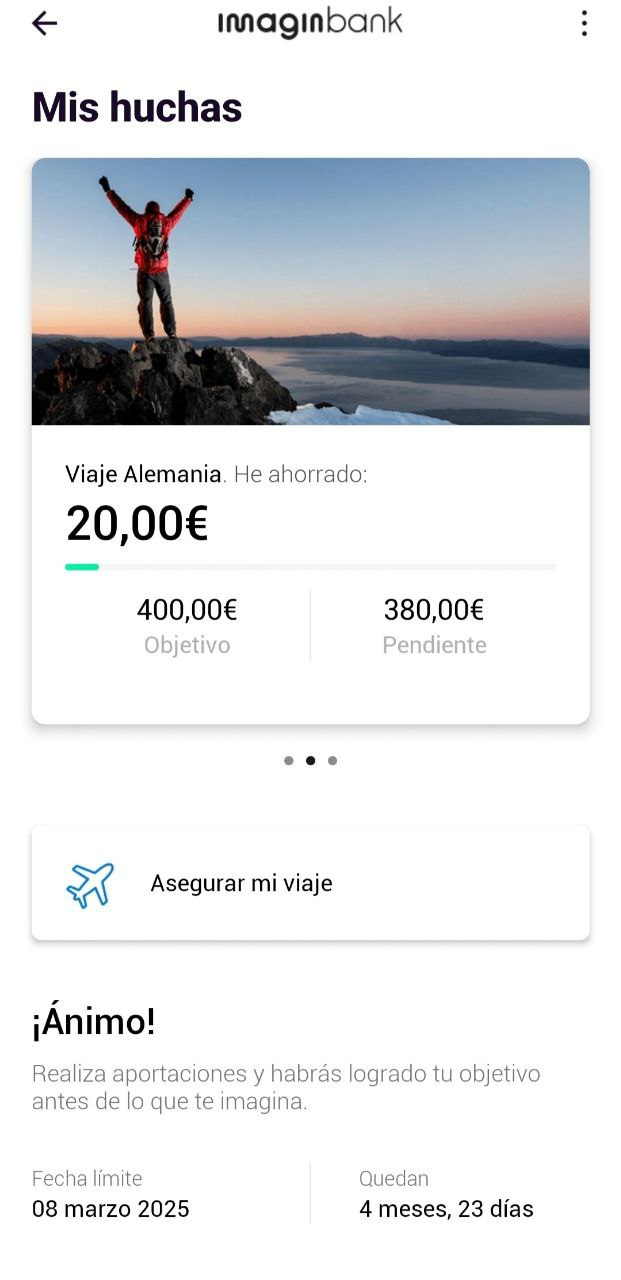
\includegraphics[height = 70mm]{imagenes/hucha-objetivo-imagin.jpg}
            \caption{Hucha de ahorro en ImaginBank\cite{hucha-imagin}.}
            \label{fig:hucha_objetivo_imagin}
        \end{minipage}\hfill
        \begin{minipage}{0.45\textwidth}
            \centering
            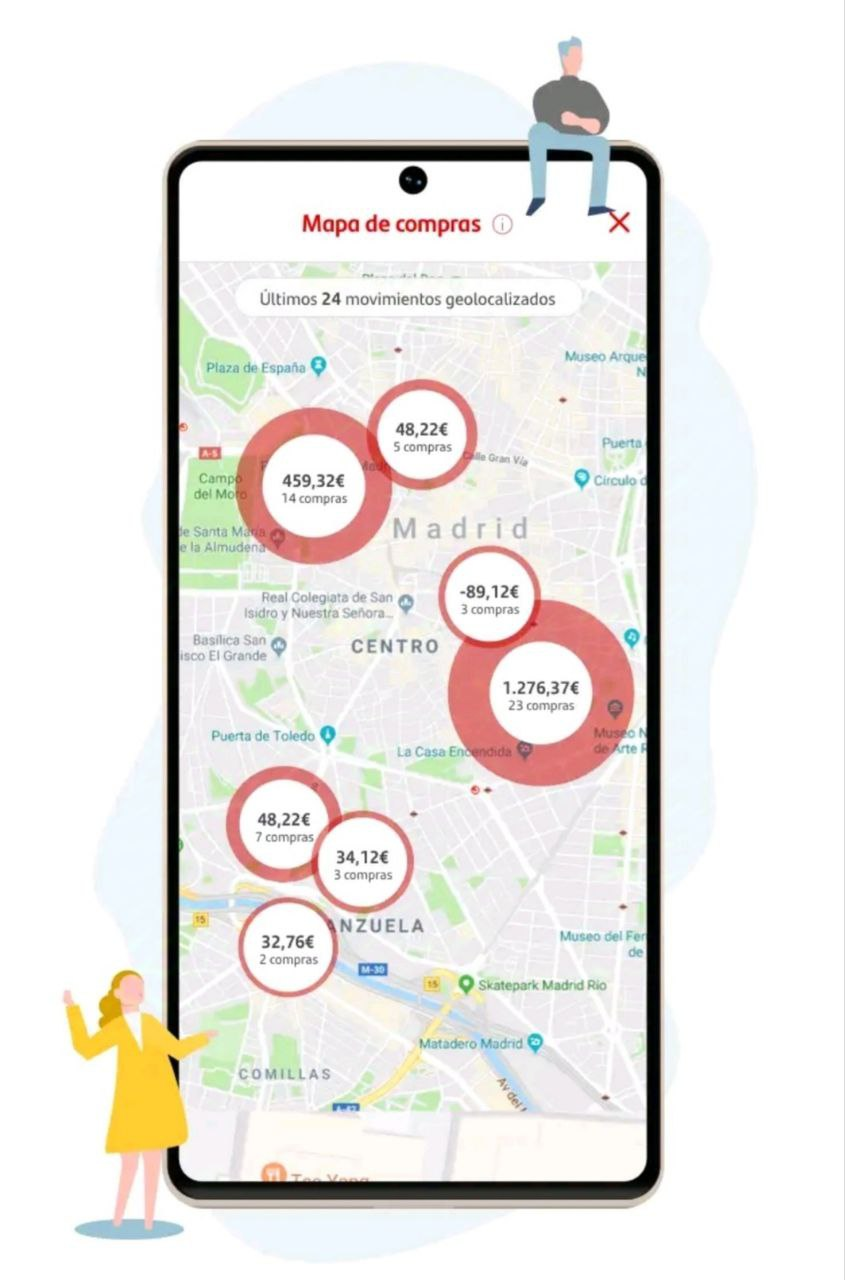
\includegraphics[height = 70mm]{imagenes/mapa-compras-santander.jpg}
            \caption{Mapa de compras en Banco Santander\cite{mapa-santander}.}
            \label{fig:mapa_compras_santander}
        \end{minipage}
    \end{figure}

    \item \textbf{BBVA}\\
    Esta última parece ser la más completa en cuanto a opciones de ahorro y análisis de gastos.

    Con \textit{Mi día a día} \footnote{\url{https://www.bbva.es/personas/banca-online/control-gastos-mi-dia-a-dia.html}}  
    obtenemos, al igual que en el resto de aplicaciones, el resumen con los movimientos de la cuenta.
    Respecto a los métodos para ahorrar existe una cuenta gratuita denominada 
    cuenta metas \footnote{\url{https://www.bbva.es/personas/productos/cuentas/cuenta-ahorro-metas.html }} 
    en la que apartar dinero a modo de hucha para conseguir hasta un máximo de 5 objetivos. 

    El apartado Presupuestos \footnote{\url{https://www.bbva.es/general/salud-financiera/economia-domestica/gestor-de-gastos-y-presupuestos.html }} 
    es el lugar donde definir una cantidad máxima de gasto deseada 
    al mes y por categoría, mide con códigos de colores la evolución del consumo 
    respecto al presupuesto. Ver figura \ref{fig:mapa_compras_santander}.
    
    \begin{figure}[ht!]
    \centering
    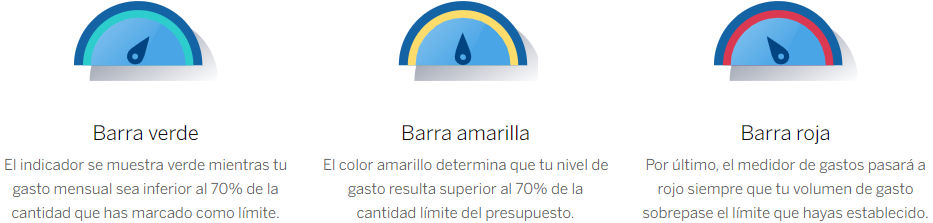
\includegraphics[height = 32mm]{imagenes/indicador_presupuestos_BBVA.png}
    \caption{Indicador de gastos respecto a presupuestos en la aplicación de BBVA
    \cite{presupuestos-BBVA}.}
    \label{fig:indicador_presupuestos_BBVA}
    \end{figure}

    Encontramos también Apartados 
    \footnote{\url{https://www.bbva.es/finanzas-vistazo/tu-guia-bbva/app/apartados-una-nueva-forma-de-ahorrar.html}}
    donde el objetivo es el mismo que en presupuestos, con la diferencia de 
    que es un espacio para separar visualmente tu dinero según tus necesidades,
    apartando la cantidad que quieras para cada tipo de gasto.

    Además, pone a disposición de los usuarios un uso parcial de la aplicación sin necesidad 
    de ser cliente, importando los datos de otros bancos (solo incluye el 
    servicio \textit{Mi día a día}).

\end{itemize}

Las aplicaciones bancarias, aunque permiten ver un resumen mensual de los gastos o 
incluso por categorías, en general no se pueden personalizar demasiado. Algunos 
métodos de ahorro llamativos por el poco esfuerzo pero ahorro constante que supone sobre el 
usuario, proponen acumular de manera automática los céntimos de euro que sobran al 
redondear cada compra en una cuenta de ahorro virtual. 

A pesar de que se están incluyendo opciones para importar los datos de movimientos de 
cuentas externas al banco, las configuraciones que se hacen dentro de 
la aplicación bancaria generalmente no se pueden exportar a otras aplicaciones.
Si se quiere cambiar de banco se pierde toda la información 
y con ella los planes de ahorro o presupuestos personalizados.

\subsection{Aplicaciones de terceros}
Por otro lado, existen \textbf{aplicaciones de terceros} que permiten unificar los gastos 
independientemente del banco al que pertenezca el usuario. Entre las más conocidas 
encontramos:

\begin{itemize}
    \item \textbf{Fintonic} \footnote{\url{https://www.fintonic.com/es-ES/inicio/}} \\
    El usuario agrega las cuentas bancarias que desee para que la aplicación 
    acceda a los datos relacionados con los movimientos de la cuenta. 
    Un aspecto que puede causar cierta reticencia es que para ello Fintonic necesita
    las claves de acceso a la cuenta bancaria (para lectura de datos).
    Tiene una interfaz intuitiva y recoge, clasifica y analiza los gastos.
    Introduce los datos de manera automática por medio de las claves proporcionadas. 
    Gratuito, con publicidad. Ver figura \ref{fig:resumen_gastos_mes_fintonic}.

    \item \textbf{Money Manager}  \footnote{\url{https://www.realbyteapps.com//}} \\
    Solo se encuentra disponible en inglés. Ofrece una gran cantidad de opciones
    para analizar gastos e incluye la opción de añadir fotos de las transacciones. 
    Se deben introducir los datos manualmente. 
    Dispone de una versión gratuita con funciones básicas.

    \item \textbf{Bluecoins} \footnote{\url{https://www.bluecoinsapp.com/}} \\
    Plantea una estructura interesante para mayor detalle de presupuestos. 
    Se pueden configurar presupuestos por categorías y subcategorías relacionadas, por ejemplo 
    los gastos del coche, se pueden separar en gasolina, seguro, mantenimiento, etc. 
    Permite añadir gastos manualmente o importarlos desde un archivo CSV y especificar 
    el tipo de pago si es en efectivo o digital, sin embargo no distingue de forma clara la cantidad por tipo de pago a la hora de realizar el gráfico resumen, como se puede ver en la figura \ref{fig:resumen_gastos_bluecoins}.
    \footnote{Un fichero CSV (\textit{Comma Separated Values}) es un archivo de texto plano 
    que almacena los datos en forma de tabla, siendo cada línea del archivo una fila y 
    cada valor un campo de dicha fila. Los campos de la fila se separan entre sí por comas 
    u otro signo de puntuación.}. 
    Ofrece versión gratuita con anuncios, de funcionalidad limitada.

    \item \textbf{Mint} \footnote{\url{https://mint.intuit.com/}} \\
    Solo se encuentra disponible en inglés. Permite vincular cuentas bancarias, tarjetas, etc. para monitorizar de forma 
    automática los gastos e ingresos. Facilita la creación de presupuestos personalizados y 
    alerta al usuario cuando se acerca a sus límites de gasto.
    En base al ritmo de ahorro estima el progreso hacia el objetivo, dando recomendaciones 
    como guía para lograrlo y gestionar el dinero de manera responsable. 
    La aplicación es gratuita con algunas limitaciones e incluye publicidad.
\end{itemize}

\begin{figure}[ht!]
    \centering
    \begin{minipage}{0.45\textwidth}
        \centering
        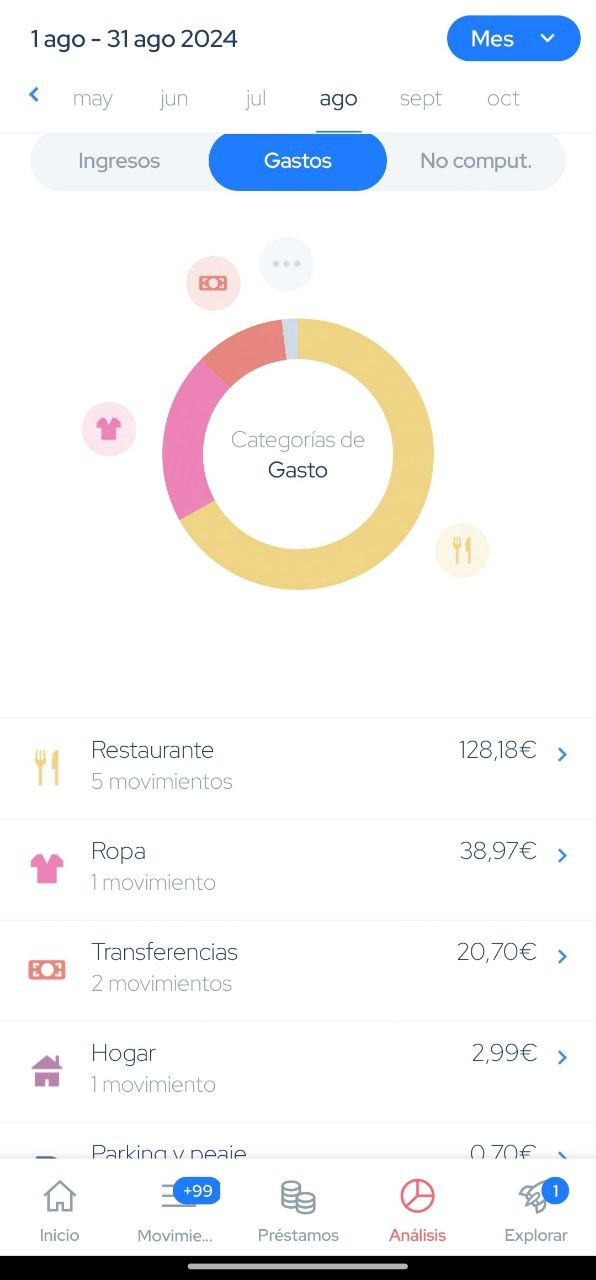
\includegraphics[height = 70mm]{imagenes/resumen-gastos-mes-fintonic.jpg}
        \caption{Resumen de gastos en Fintonic\cite{gastos-fintonic}.}
        \label{fig:resumen_gastos_mes_fintonic}
    \end{minipage}\hfill
    \begin{minipage}{0.45\textwidth}
        \centering
        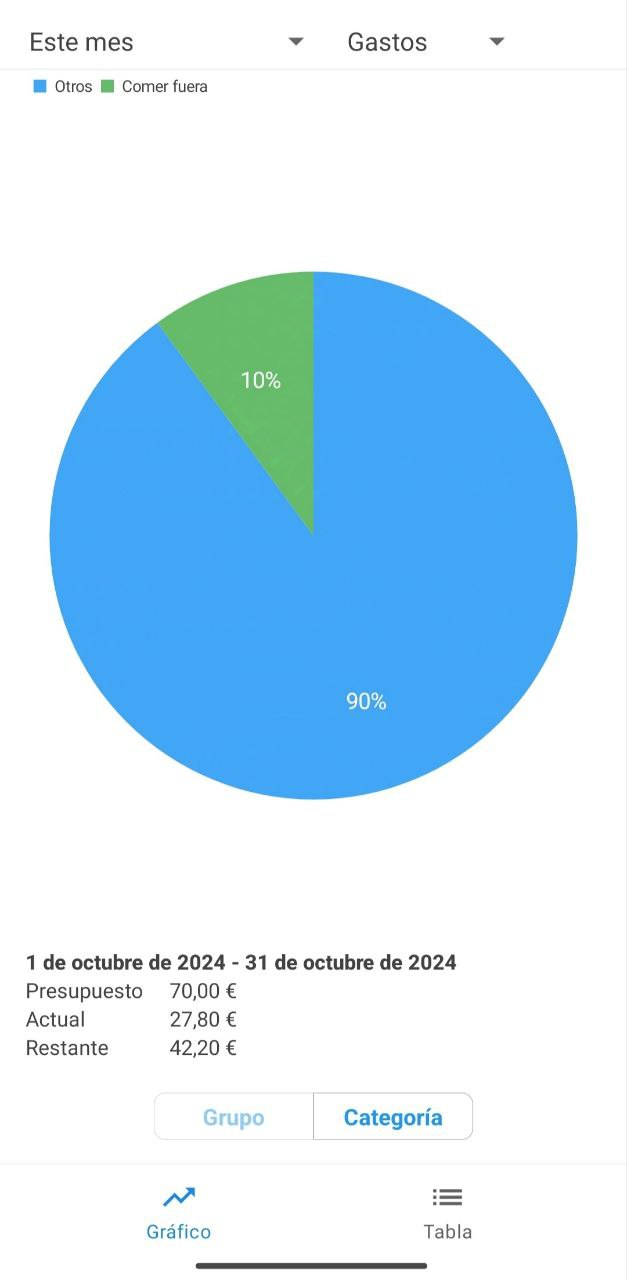
\includegraphics[height = 70mm]{imagenes/resumen-gastos-bluecoins.jpg}
        \caption{Resumen de gastos en Bluecoins\cite{gastos-bluecoins}.}
        \label{fig:resumen_gastos_bluecoins}
    \end{minipage}
\end{figure}

Además existen aplicaciones de gestión avanzada como \textbf{Pleo} 
\footnote{\url{https://www.pleo.io/es}}, que ofrece una solución para la gestión 
de gastos de empresa. Dispone de una tarjeta 
de empresa que se puede usar para pagar gastos y que se sincroniza con la aplicación 
para agilizar la contabilidad entre los empleados y la empresa. 
Entre otras características ofrece análisis útiles para el administrador en la empresa 
y permite a los empleados justificar los gastos al pedirles añadir foto del ticket recibido. 
Ver figura \ref{fig:resumen_gastos_pleo}.
\begin{figure}[ht!]
    \centering
    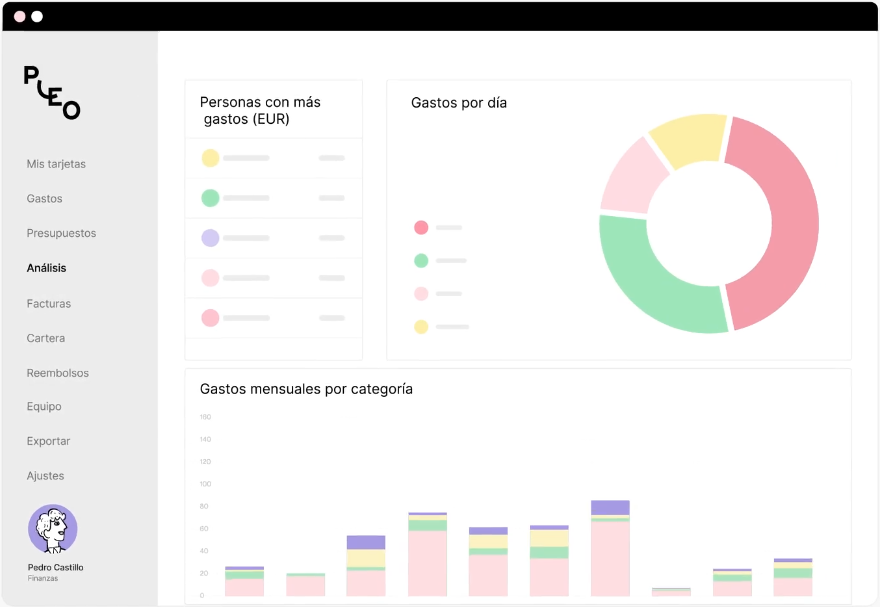
\includegraphics[width = 90mm]{imagenes/resumen-gastos-pleo.png}
    \caption{Resumen de gastos de empleados \cite{gastos-pleo}.}
    \label{fig:resumen_gastos_pleo}
\end{figure}


\subsection{Proyectos académicos}
Proyectos académicos relacionados con el ámbito de la gestión y la educación financiera.

\begin{itemize}
    \item \textbf{Sevilla Borja, Kevin Paúl}. 
    \textit{Aplicación móvil para fomentar la educación financiera en las finanzas personales 
    de los estudiantes de la PUCESA} (universidad de Ecuador) \cite{sevilla2024aplicacion}. \\
    Orientada a mejorar la capacidad
    de gestionar eficazmente las finanzas personales de los estudiantes. La aplicación 
    permite llevar un control básico de ingresos y gastos. Su característica más significativa 
    es la oferta de módulos educativos en la propia aplicación sobre conceptos financieros, como 
    ayuda para reforzar su confianza en la toma de decisiones.

    \item \textbf{Tamayo Valdivielso, Pablo}. 
    \textit{Budger: desarrollo de una app financiera} \cite{tamayo2022aplicacion}. \\ 
    Este producto desarrollado como 
    trabajo final de máster de desarrollo de aplicaciones móviles, consiste en una aplicación 
    con la que ayudar a los usuarios a controlar su dinero de una forma sencilla. Incluye 
    gráficos para visualizar el resumen de los datos y 
    permite la creación de un presupuesto global de gastos que parte del resto de los ingresos 
    que no se dedicarán a ahorro, fomentando de esta manera la planificación del usuario.

    \item \textbf{García García, Felicidad}. 
    \textit{Tus finanzas personales} \cite{garcia2019aplicacion}. \\  
    Aplicación móvil para dispositivos Android, 
    desarrollada como trabajo de fin de máster para la gestión de las finanzas personales. 
    Con finalidad de ayudar al usuario a priorizar sus gastos necesarios sobre aquellos
    que no lo son establece una clasificación de gastos en función de su importancia. 
    Los gastos se puden introducir de manera manual o permitir la incorporación de 
    movimientos bancarios accediendo a las cuentas del usuario con permiso explícito para ello.
    
\end{itemize}

\section{Conclusiones}
Tras repasar las soluciones discutidas anteriormente, encontramos numerosas 
características útiles dentro de las aplicaciones para ayudar a la gestión 
de los gastos. Algunas de ellas con más fortaleza en las secciones de análisis, 
otras en la automatización (como las que permiten la importación de datos bancarios) y  
otras, por ejemplo, en la personalización. 

Teniendo en cuenta las características generalizadas de las diferentes soluciones, 
obtenemos la siguiente tabla comparativa de esfuerzo por parte del usuario. Ver 
tabla \ref{tab:comparativa_soluciones}.

El esfuerzo del usuario depende, en gran medida, de la aplicación y la funcionalidad concreta que necesite. Por este motivo, este proyecto surge con la idea de crear una aplicación enfocada en la gestión unificada de movimientos monetarios, para ayudar al usuario a planificar y vigilar sus gastos y ahorros independientemente de la fuente de la que provengan dichas transacciones, pero 
sin dejar de lado de la automatización y personalización al incluir los datos.


\begin{landscape}
\begin{table}[]
\begin{tabular}{|l|l|l|l|l|}
\hline
& \textbf{Tradicional} & \textbf{\begin{tabular}[c]{@{}l@{}}Aplicaciones\\ bancarias\end{tabular}} & \textbf{Aplicaciones de terceros} & \textbf{\begin{tabular}[c]{@{}l@{}}Proyectos\\ académicos\end{tabular}} \\ \hline
\textbf{\begin{tabular}[c]{@{}l@{}}Anotación de movimientos\\ (gastos, ingresos y ahorros)\end{tabular}} & Alto & Muy bajo & \begin{tabular}[c]{@{}l@{}}Con integración banco: Muy bajo\\ Sin integración banco: Medio - Alto\end{tabular} & Medio - Alto \\ \hline
\textbf{Control de dinero efectivo} & Alto & No tienen & \begin{tabular}[c]{@{}l@{}}Con integración banco: No tiene\\ Sin integración banco: Medio\end{tabular} & Medio \\ \hline
\textbf{Control de dinero digital} & Alto & Bajo & Bajo & Bajo \\ \hline
\textbf{\begin{tabular}[c]{@{}l@{}}Creación de categorías de\\ gastos (con presupuestos)\end{tabular}} & Alto & \begin{tabular}[c]{@{}l@{}}No personalizable\\ (automático)\end{tabular} & Medio - Bajo & Bajo \\ \hline
\textbf{\begin{tabular}[c]{@{}l@{}}Creación de objetivos de\\ ahorro\end{tabular}} & Alto & \begin{tabular}[c]{@{}l@{}}Bajo (nº limitado\\ de objetivos)\end{tabular} & \begin{tabular}[c]{@{}l@{}}Con integración banco: No tienen\\ Sin integración banco: Medio\end{tabular} & \begin{tabular}[c]{@{}l@{}}No tienen (lo que no\\ se gasta se considera\\ ahorro)\end{tabular} \\ \hline
\textbf{Resúmenes de gastos totales} & Alto & Muy bajo & Muy bajo & Muy bajo \\ \hline
\textbf{\begin{tabular}[c]{@{}l@{}}Representación gráfica\\ de gastos\end{tabular}} & Medio - Alto & Muy bajo & Muy bajo & Muy bajo \\ \hline
\textbf{\begin{tabular}[c]{@{}l@{}}Representación gráfica\\ de ahorros\end{tabular}} & Medio - Alto & No tienen & Muy bajo & Muy bajo \\ \hline
\textbf{Personalización} & Bajo & Medio - Alto & \begin{tabular}[c]{@{}l@{}}Con integración banco: Alto\\ Sin integración banco: Medio\end{tabular} & Bajo \\ \hline
\end{tabular}
\label{tab:comparativa_soluciones}
\caption{Comparativa de esfuerzo por parte del usuario en las diferentes soluciones.}
\end{table}
\end{landscape}


	
	\chapter{Planificación}

La planificación en el desarrollo de un proyecto es un aspecto clave para organizar las tareas, trabajar de manera eficiente y garantizar el cumplimiento de plazos y objetivos.

\section{Metodología utilizada}
Las metodologías ágiles son un enfoque flexible y adaptativo para la gestión de proyectos, especialmente en desarrollo de software. Entre otros, se caracterizan por iteraciones cortas, aceptación del cambio en los requisitos durante el desarrollo y entregas continuas de producto (con el objetivo de satisfacer al cliente con software de valor desde el inicio)\cite{agileprinciples}.

\textit{Kanban} es un enfoque ágil que destaca por la gestión visual del flujo de trabajo. Utiliza un tablero con columnas que representan diferentes etapas del proceso (como el trabajo realizado, lo que está en proceso y tareas futuras). Los elementos del proyecto se mueven a lo largo del tablero; esto facilita al desarrollador trabajar de acuerdo al enfoque de Kanban: el desarrollador se centra en limitar las tareas en progreso para mejorar la productividad y evitar la sobrecarga\cite{majkamastering}.

Se ha optado por el uso de \textit{Kanban} por su flexibilidad y simplicidad. Permite gestionar el proyecto sin imponer plazos fijos, algo útil cuando trabajas solo y necesitas adaptar tu ritmo según las circunstancias y la carga de trabajo. Además de la gestión visual, Kanban, al facilitar la priorización de tareas y la realización de entregas continuas, permite avanzar hacia objetivos bien definidos.

Existen herramientas de gestión de proyectos que nos facilitan la implementación de esta metodología, como \textit{Trello}\footnote{\url{https://trello.com/es}} o \textit{Click Up}\footnote{\url{https://clickup.com/es-ES}}, con tableros personalizados y colaborativos para organizar tareas de proyectos.


\section{Temporización}
Siguiendo el enfoque \textit{Kanban}, se ha establecido un tablero (como se puede ver en la Figura \ref{fig:tablero_kanban}) con las tareas a realizar en el proyecto. Se definen hitos de desarrollo cuyo cumplimiento supone el final de un milestone (definición de milestones en el capítulo de análisis\ref{sec:milestones}) y el inicio del siguiente; los milestones (o hitos) incluirán un desglose de tareas, que podrán incluir la implementación de funcionalidades, resolución de problemas encontrados y realización de pruebas. 

De esta forma el final del milestone se puede marcar con la finalización de todas las tareas asociadas a él, lo que supone un producto entregable funcional y de valor para el cliente. 

Los milestones guían la planificación del proyecto y permiten el seguimiento temporal del mismo, están sujetos a cambios según las necesidades del proyecto.

\begin{figure}[ht!]
    \centering
    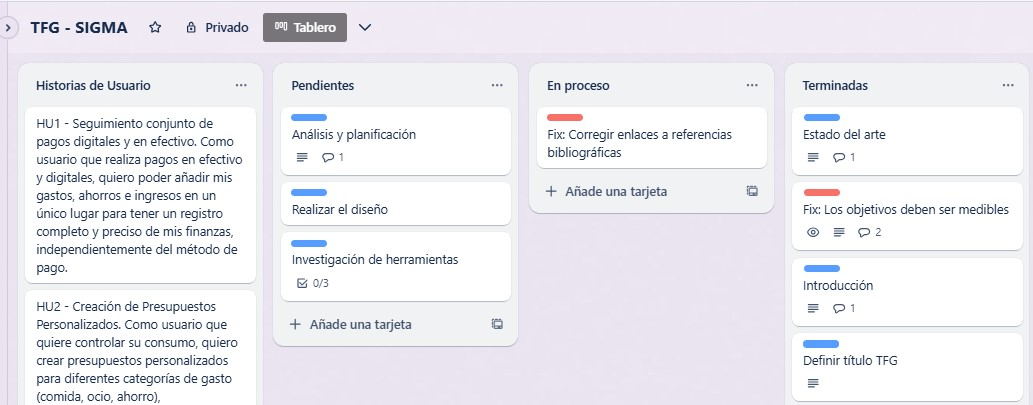
\includegraphics[width=\linewidth]{imagenes/tablero_kanban.jpg}
    \caption{Captura de pantalla del tablero kanban en \textit{Trello}.}
    \label{fig:tablero_kanban}
\end{figure}


\section{Costes}
En este capítulo se describen los recursos y materiales usados en el desarrollo del proyecto, junto con los costos asociados a cada uno de ellos.

\subsection{Recursos humanos}

En el desarrollo de la aplicación web \textit{SIGMA}, se ha contado con un desarrollador que ha hecho también las labores de diseño para la interfaz y redacción de este documento.

\subsection{Hardware y software}
Como recursos materiales, han sido utilizados un ordenador personal portátil y un monitor (Tabla \ref{tab:costes-hardware}),
propiedad del desarrollador, los cuales han sido de gran utilidad para las tareas de diseño y desarrollo al permitir el visionado de diferentes recursos simultáneamente.

\begin{table}[H]
    \begin{center}
    \begin{tabular}{| l | c | c | c |}
        \hline
        \textbf{Hardware} & \textbf{Coste} \\ \hline
        Acer Extensa 2511 & 589\euro \\
        Monitor LG & 132,68\euro \\ \hline
        \textbf{Coste total hardware}: & \textbf{721,68\euro} \\ \hline
    \end{tabular}
    \caption{Coste de materiales hardware.}
    \label{tab:costes-hardware}
    \end{center}
\end{table} 

Para desarrollar este proyecto no se ha usado ningún software ni biblioteca de pago con el propósito de reducir costes, por lo que el software externo no incrementa el coste final. Por otro lado, el coste del hardware anteriormente mencionado, viene condicionado por la vida útil estimada de los dispositivos. En el caso de un ordenador portátil y un monitor, se estiman entre 5 y 7 años (en buenas condiciones)\cite{tecfys2023}.
\begin{equation}
    \textbf{Coste Anual} = \frac {\text{Coste Hardware}}{\text{5 años}} = \text{144,336 €/año}
\end{equation}

\begin{equation}
    \textbf{Coste Mensual} = \frac {\text{Coste Anual}}{\text{12 meses}} = \text{12,03 €/mes}
\end{equation}

\begin{equation}
    \textbf{Materiales x N Meses} = \text{Coste Mensual/mes} \times \text{8 meses} = \text{96,224 €}
\end{equation}

\subsection{Presupuesto sobre profesionales implicados}
En esta sección se detallarán los costos del proyecto. Se considerará el perfil de un puesto junior de desarrollador \textit{fullstack}, cuyo salario anual oscila entre los 17.000€ y 22.000€ \cite{glassdoor2024}.
Teniendo en cuenta que la implementación ha tomado un tiempo aproximado de 370 horas, se puede calcular un coste estimado del salario del desarrollador, el cual se detalla a continuación:

\begin{equation}
    \textbf{Salario medio fullstack junior} =  \frac {\text{19.500 €/año} }{ \text{12 meses}} = \text{1.625 €/mes}
\end{equation}

El salario por hora se calcula dividiendo el salario mensual entre 160 horas, que es el promedio de horas laborales al mes:

\begin{equation}
    \textbf{Salario por hora} = \frac {\text{1.625 €/mes}}{160 \text{ horas}} = \text{10,16 €/hora}
\end{equation}

Teniendo en cuenta las 370 horas de trabajo, se puede calcular el coste total del salario:

\begin{equation}
    \textbf{Coste total salario} = \text{370 horas} \times \text{10.16 €/hora} = \text{3.757,81 €}
\end{equation}

Para el diseño, se tendrá en cuenta el perfil de un diseñador gráfico, cuyo salario medio es de unos 18.180 € \cite{glassdoor-dis-grafico-2024}. Teniendo en cuenta que el diseño ha supuesto un aproximado de 30 horas. Partiendo de esta información, se puede calcular el coste total del salario del diseñador, el cual se detalla a continuación:

\begin{equation}
    \textbf{Salario medio diseñador gráfico} =  \frac {\text{18.180 €/año} }{ \text{12 meses}} = \text{1,515 €/mes}
\end{equation}

El salario por hora se calcula dividiendo el salario mensual entre 160 horas, que es el promedio de horas laborales al mes:

\begin{equation}
    \textbf{Salario por hora} = \frac {\text{1,515 €/mes}}{160 \text{ horas}} = \text{9,47 €/hora}
\end{equation}

Teniendo en cuenta las 30 horas de trabajo, se puede calcular el coste total del salario del diseñador:

\begin{equation}
    \textbf{Coste salario} = \text{30 horas} \times \text{9,47 €/hora} = \text{284,06 €}
\end{equation}

\subsection*{Total}

Sumando los costes asociados a los salarios y materiales usados, se obtiene el coste total aproximado del proyecto (representado en la Tabla \ref{tab:coste-total}).

\begin{table}[H]
    \begin{center}
    \begin{tabular}{| l | c | c | c |}
        \hline
        \textbf{Entidad} & \textbf{Coste} \\ \hline
        Desarrollador & 3.757,81\euro \\
        Diseñador  & 284,06\euro \\ \hline
        Hardware
        \textbf{Coste total}: & \textbf{4.041,87\euro} \\ \hline
    \end{tabular}
    \caption{Coste de materiales hardware.}
    \label{tab:coste-total}
    \end{center}
\end{table} 

	% Análisis del problema
	% 1. Análisis de requisitos
	% 2. Análisis de las soluciones
	% 3. Solucion propuesta
	% 4. Análisis de seguridad
	\chapter{Análisis del problema}
 


	% Desarrollo bajo sprints: 
	% 	1. Permitir registros y login de usuarios
	% 	2. Desarrollo del sistema de incidencias
	% 	3. Desarrollo del sistema de denuncias administrativas y accidentes
	% 	4. Desarrollo del sistema de croquis
	%   5. Instalación de la aplicación de manera automática
	\chapter{Implementación}

La implementación del software se ha dividido en hitos. Estos, han sido definidos en Github
y cada uno de ellos contiene un grupo de \textit{issues} que se corresponden con las distintas
mejoras que se han ido incorporando al software a lo largo de su desarrollo.\\



	% Presupuesto

	% Conclusiones
	\chapter{Conclusiones y trabajos futuros}

\section{Conclusiones}

CONCLUSIONES: Visión comercial?
En la actualidad, cada vez son más los comercios que ofrecen la posibilidad de recibir 
el ticket en formato digital. En un futuro probablemente todos los tickets serán 
digitales para reducir el impacto ambiental del uso del papel y abaratar costes.

Por lo que se incluirá en la aplicación la opción de escaneo de tickets digitales.


	% Trabajos futuros


	
	\newpage
	\bibliography{bibliografia}
	\bibliographystyle{plain}
	
\end{document}
